%%%%%%%%%%%%%%%%%%%%%%%%%%%%%%%%%%%%%%%%%
% Short Sectioned Assignment
% LaTeX Template
% Version 1.0 (5/5/12)
%
% This template has been downloaded from:
% http://www.LaTeXTemplates.com
%
% Original author:
% Frits Wenneker (http://www.howtotex.com)
%
% License:
% CC BY-NC-SA 3.0 (http://creativecommons.org/licenses/by-nc-sa/3.0/)
%
%%%%%%%%%%%%%%%%%%%%%%%%%%%%%%%%%%%%%%%%%

%----------------------------------------------------------------------------------------
%   PACKAGES AND OTHER DOCUMENT CONFIGURATIONS
%----------------------------------------------------------------------------------------

\documentclass[paper=a4, fontsize=11pt]{scrartcl} % A4 paper and 11pt font size

\usepackage[T1]{fontenc} % Use 10-bit encoding that has 256 glyphs
\usepackage{polski}
\usepackage[utf8]{inputenc}
\usepackage[polish]{babel}
\usepackage{amsmath,amsfonts,amsthm} % Math packages
\usepackage{pgfplots} % Math packages
\usepackage{lipsum} % Used for inserting dummy 'Lorem ipsum' text into the template
\usepackage{enumerate}
\usepackage{sectsty} % Allows customizing section commands
\usepackage{gensymb}
\usepackage{fancyhdr} % Custom headers and footers
\pagestyle{fancyplain} % Makes all pages in the document conform to the custom headers and footers
\fancyhead{} % No page header - if you want one, create it in the same way as the footers below
\fancyfoot[L]{} % Empty left footer
\fancyfoot[C]{} % Empty center footer
\fancyfoot[R]{\thepage} % Page numbering for right footer
\renewcommand{\headrulewidth}{0pt} % Remove header underlines
\renewcommand{\footrulewidth}{0pt} % Remove footer underlines
\setlength{\headheight}{13.6pt} % Customize the height of the header
\usepackage{listings}
\DeclareGraphicsExtensions{.pdf,.png,.jpg,.gif}

\pgfplotsset{compat=1.10}
\numberwithin{equation}{section} % Number equations within sections (i.e. 1.1, 1.2, 2.1, 2.2 instead of 1, 2, 3, 4)
\numberwithin{figure}{section} % Number figures within sections (i.e. 1.1, 1.2, 2.1, 2.2 instead of 1, 2, 3, 4)
\numberwithin{table}{section} % Number tables within sections (i.e. 1.1, 1.2, 2.1, 2.2 instead of 1, 2, 3, 4)

\setlength\parindent{0pt} % Removes all indentation from paragraphs - comment this line for an assignment with lots of text

%----------------------------------------------------------------------------------------
%   TITLE SECTION
%----------------------------------------------------------------------------------------

\newcommand{\horrule}[1]{\rule{\linewidth}{#1}} % Create horizontal rule command with 1 argument of height

\title{ 
    \normalfont \normalsize 
    \textsc{Politechnika Warszawska} \\ [25pt] % Your university, school and/or department name(s)
    \horrule{0.5pt} \\[0.4cm] % Thin top horizontal rule
    \huge Projekt z przedmiotu fizyczne podstawy transmisji i przechowywania informacji \\ % The assignment title
    \horrule{2pt} \\[0.5cm] % Thick bottom horizontal rule
}

\author{Mateusz Starzycki} % Your name

\date{\normalsize\today} % Today's date or a custom date

\begin{document}

\maketitle % Print the title
\newpage
\tableofcontents
\newpage
%----------------------------------------------------------------------------------------
%   PROBLEM 1
%----------------------------------------------------------------------------------------

\newpage


\section{Treść Zadania}

Wiedząc, że moc nadajnika wynosi \(P_N\), sprawność fotodiody wynosi \(X\), zaprojketuj jak najdłuższe łącze światłowodowe jednokanałowe
(działające w trzecim oknie telekomunikacyjnym) o przepływności B (nie używając wzmacniaczy). Załóż że straty na spawach i połączeniach wynoszą odpowiednio
\(A_s\) - 1 spaw i \(A_c\) - 1 złącze. Wybierz trzy różne odległości między spawami z przedziału [5;10] km. Omów wpływ odległości między spawami na zasięg łącza.
Potrzebne parametry włókna światłowodowego znajdź na stronie producenta. Omów poszczególne etapy projektu i wpływ parametrów łącza na jego zasięg.

\begin{tabular}{ | c | c | c | c | c | c | c | }
    \hline
    \(L_P\) & \(P_N [mW] \) & \(X[\%]\) & \(A_S[dB]\) & \(A_C[dB]\) & \(B[Gb/s]\) & Imię i Nazwisko \\
    \hline
    35 &  9 & 80 & 0.15 & 0.5 & 9 & Mateusz Starzycki \\
    \hline
\end{tabular}

\section{Teoria transmisji światłowodowej}

\subsection{Wstęp}

Transmisja światłowodowa jest to przesył informacji za pomocą wiązki elektromagnetycznej z zakresu fal widzialnych.
Sygnał przesyłany jest przy użycia nosnika który utrzymuje w sobie falę przy wykorzystaniu całkowitego wewnętrznego odbicia.
Nośnik taki nazywamy światłowodem.
Aby możliwe było powstanie tego zjawiska swiatłowód musi zostać wykonany z przynajmniej dwóch ośrodków o róznej prędkości propagacji światła.

\subsection{Zjawiska występujące w Światłowodzie}

W światłowodzie zachodzi wiele zjawisk fizycznych, można je podzielić na zjawiska porządane i negatywnie wpływające na transmisję sygnału.

\subsubsection{Całkowite wewnętrzne odbicie}

Najważniejszym, porządanym zjawiskiem jest opisane we wstępnie zjawisko całkowitego wewnętrznego odbicia. Polega ono na odbiciu promienia świetlnego od
krawędzi dwóch ośrodków bez możliwości przeniknięcia do drugiego ośrodka. Aby zjawisko to miało miejsce muszą zostać spełnione dwa warunki:
\begin{itemize}
  \item Ośrodek w którym światło się znajduje musi mieć większy współczynnik załamania niż ośrodek od którego odbija się światło.
  \item Kąt padania musi być większy od pewnego kąta krytycznego.
\end{itemize}

Kąt krytyczny jest to taki kąt w którym wiązka odbijająca się w granicy dwóch ośrodków musiałaby po odbiciu przebiegać wzdłóż granicy ośrodków.
Można zwizualizować to na następującym schemacie:

Z prawa załamania można obliczyć zatem kąt odbicia.\[n_1sin\Theta_1=n_2sin\Theta_2\] 
Podkładając \[\Theta_{gran}=90\degree\] 
Otrzymujemy: \[n_1sin\Theta_C=n_2sin\Theta_{gran}\]
Po przekształceniu możemy wyliczyć kąt graniczny z wzoru \[\Theta_C=arcsin\frac{n_2}{n_1}\]

Zjawisko to jest wykorzystywane w światłowodzie gdyż sprawia iż sygnał jest całkowicie "uwięziony" w wiązce, pod warunkiem że wpada do niego
z odpowiednim kątem i pod warunkiem że światłowód nie jest mocno zgięty w żadnym fragmencie.

\subsubsection{Tłumienie}

W związku z tym iż nośnikiem informacji są fotony o określonej długości fali, na drodze światła dochodzi do jego rozproszenia przez jądra atomowe oraz absorpcji poprzez
elektrony. Zjawisko to powoduje osłabienie sygnału w zależności od przebytej drogi w światłowodzie. 

Intensywność absorpcji fotonów zależy od długości fali i jest ustalone przez rodzaj wykorzystanego źródła sygnału w światłowodzie. Następujący rysunek prezentuje
zależność absorpcji (uwzględniający oba zjawiska) od długości fali. Na rysunku zostały naniesione linie (od lewej) intensywności rozproszen Rayleight'a oraz absorpcji podczerwieni.

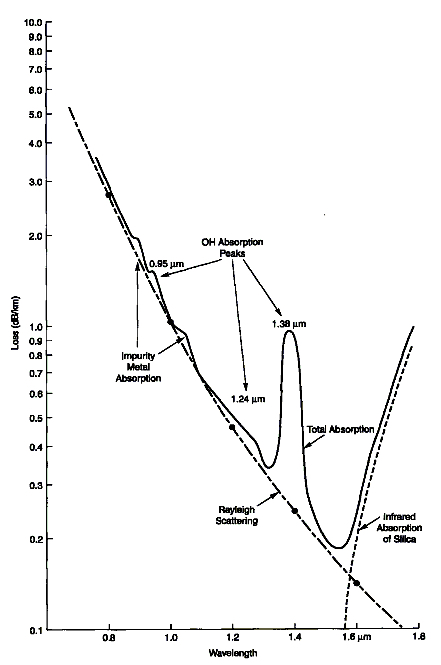
\includegraphics[width=\textwidth]{1}

Tak jak pokazano na rysunku, stosowane światłowody znajdują się w trzech oknach długości fali.

\subsubsection{Straty na złączach i spawach}

Dodatkowymi czynnikami tłumienia są niedoskonałości wykonania światłowodu. Zjawiska takie występują miedzy innymi na złaczach końcowych oraz spawach pomiędzy
fragmentami światłowodów, ma to związek z lokalnymi zaburzeniami geometrii które są dużo większe niż w innych miejscach światłowodu.

\subsubsection{Dyspersja}

Dodatkowym zjawiskiem występującym w światłowodzie jest dyspersja. Zjawisko to występuje z powodu różnicy dróg przebytej przez poszczególne fale.
W związku z tym iż odbijają się one wielokrotnie od krawędzi światłowodu początkowo prostokątny sygnał intensywności w funkcji czasu zostaje rozmyty.
Jego ostre krawędzie zostają rozmyte w czasie. Rysunek przedstawia zjawisko dyspersji, wykres intensywności sygnału w czasie w oddalających się od źródła
fragmentach światłowodu.

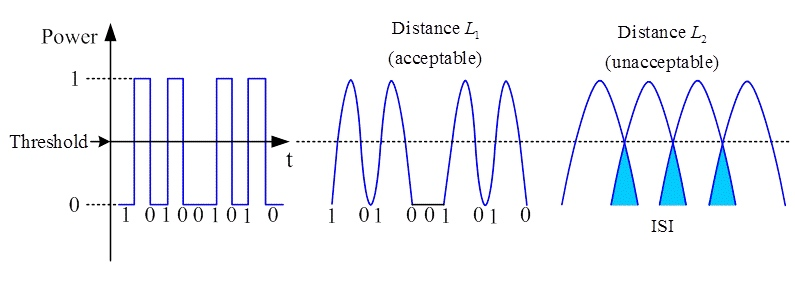
\includegraphics[width=\textwidth]{2}

Wymieniona dyspersja dotyczy wielomodowych światłowodów. W przypadku jednomodowego nie jest możliwa propagacja innymi drogami.

Drugim przykładem dyspersji jest dyspersja spowodowana zależnością prędkości grupowej od długości fali.
Współczynnik dyspersji opisuje jak bardzo rozszerza się sygnał w zależności od czasu propagacji.

Ostatnim rodzajem dyspersji jest dyspersja polaryzacyjna polegająca na różnej prędkości propagacji ortogonalnych wiązek promieniowania elektromagnetycznego.
  
\subsection{Wzory do obliczania stratności}

W celu obliczenia maksymalnej długości światłowodu należy dokonać cyklu obliczeń które pozwolą oszacować bilans tłumienia w połączeniu.
Obliczenia te uwzględniają własności układu w którym znajdzie się światłowód oraz jego fizyczne właściwości.

\subsubsection{Intensywność na wejściu}

Pierwszym krokiem jest ustalenie jaka jest intensywność (moc) sygnału który dotrze do światłowodu. Zależy on od mocy układu elektrycznego zasilającego
fotodiodę oraz sprawności fotodiody.

W celu obliczenia mocy wejściowej należy wykorzystać następujący wzór:
\begin{equation} \label{eq:moc} 
P_w = P_N \cdot X
\end{equation}
Gdzie:\\
\par \setlength\parindent{24pt}
\(P_w\) - Moc nadajnika\\
\par \setlength\parindent{24pt}
\(X\) - sprawność fotodiody\newline

\subsubsection{Tłumienie całkowite}

Tłumienie jest to wartość w db podająca jaki jest stosunek sygnału wyjściowego do wejściowego. W celu obliczenia całkowitego tłumienia należy zsumować
tłumienia cząstkowe powstałe w wyniku : złącz końcowych, spawów, tłumienia w światłowodzie.
Całkowite tłumienie można zatem wyrazić przy pomocy wzoru:
\begin{equation} \label{eq:sprawnosc} 
  A_{calk} = 2\cdot A_C + k \cdot A_S + n \cdot A_F
\end{equation}\\
Gdzie:\\
\par \setlength\parindent{24pt}
\(A_{calk}\) - tłumienie całkowite\\
\par \setlength\parindent{24pt}
\(A_C\) - tłumienie złącz\\
\par \setlength\parindent{24pt}
\(k\) - ilość spawów (nieznana)\\
\par \setlength\parindent{24pt}
\(A_S\) - tłumienie spawu\\
\par \setlength\parindent{24pt}
\(n\) - długość światłowodu w km (nienzane)\\
\par \setlength\parindent{24pt}
\(A_F\) - tłumienie światłowodu na kilometr\newline


Należy pamiętać iż tłumienie musi być dobrane do odpowiedniej długości fali światła (dla 3 okna jest to 1550 nm).

Ilość spawów oraz długość światłowodu nie są znane, wartości te można uzależnić w następujący sposób:
\begin{equation} \label{eq:iloscodc} 
  k = \frac{n}{l_f}
\end{equation}
Gdzie \(l_f\) to długość fragmentu światłowodu ( w treści zadania nalęży wybrać 3 z przedziłu 5-10 km).
Wybrane wartości to 5; 7.5 oraz 10.

\subsubsection{Moc niezbędna}

Moc niezbędna jest to minimalna moc potrzebna na zapewnienie zadanej przepustowości złącza. Moc wyjściowa niezbędna opisana jest
poprzez czułość odbiornika. Czułość odbiornika określa następująca zależność: 

\begin{equation} \label{eq:czulosc} 
  P_R = \frac{n_0hfB_0}{10^{-3}}
\end{equation}
\\
Gdzie:\\
\par \setlength\parindent{24pt}
\(P_R\) - czułość odbiornika\\
\par \setlength\parindent{24pt}
\(n_0\) - liczba fotonów na bit (założono 300)\\
\par \setlength\parindent{24pt}
\(h\) - stała Plancka\\
\par \setlength\parindent{24pt}
\(f\) - częstotliwość fali\\
\par \setlength\parindent{24pt}
\(B_0\) - przepustowość łącza\newline

\subsubsection{Moc wyjściowa}

\par Moc wyjściowa sygnału jest to nic innego jak moc wejściowa po osłabieniu przez tłumienie wynosi ona:

\begin{equation} \label{eq:mocwyjsc} 
  10log_{10}\frac{P_w}{P_e} = A_{calk}
\end{equation}

\subsubsection{Dyspersja}

Wzory na dyspersję zostały podane przez producenta.
Dwa występujące zjawiska dyspersji to dyspersja polaryzacyjna:

\begin{equation}
  D_p = \sqrt{l} \cdot S_d
\end{equation}
Gdzie:\\
\par \setlength\parindent{24pt}
\(l\) - długość światłowodu\\
\par \setlength\parindent{24pt}
\(S_d\) - współczynnik dyspersji\\

Oraz dyspersja chromatyczna:

\begin{equation}
  D(\alpha)=\frac{s_0}{4}[\alpha-\frac{\alpha_0^4}{\alpha^3}] \cdot l
\end{equation}
Gdzie:\\
\par \setlength\parindent{24pt}
\(\alpha\) - długość fali efektywna (1550nm)\\
\par \setlength\parindent{24pt}
\(\alpha_0\) - długość fali dispersyjnej (1302nm) \\
\par \setlength\parindent{24pt}
\(\S_0\) - współczynnik dyspersji \\
\par \setlength\parindent{24pt}
\(l\) - długość światłowodu\\


\section{Obliczenia}

\subsection { Wstęp }

W celu obliczenia maksymalnej możliwej długości należy znaleść maksymalne rozwiązanie następującej nierówności:

\begin{equation} \label{eq:problem} 
  P_e \ge P_R 
\end{equation}

Warto zauważyć iż będzie to tylko teoretycznie możliwa do uzyskania długość, zwykle należy przemnożyć wszystko przez
współczynnik bezpieczeństwa. Dodatkowo warto zauważyć że ze wzrostem długości łącza tłumienie będzie jedynie rosnąć, 
a co za tym idzie moc wyjściowa będzie maleć, w związku z czym można zredukować nierówność do przypadku gdy obie te moce są
równe, będzie to maksymalna możliwa do utrzymania długość złącza.

\subsection {Rozwiązanie problemu}

\subsubsection { Przekształcenia wzorów }

Podstawiając \eqref{eq:problem}  do \eqref{eq:mocwyjsc} otrzymujemy:

\begin{equation} 
  10log_{10}\frac{P_w}{P_R} = A_{calk}
\end{equation}

Następnie podstawiając \eqref{eq:moc}
\begin{equation} 
  10log_{10}\frac{P_N \cdot X}{P_R} = A_{calk}
\end{equation}

Następnie podstawiając \eqref{eq:czulosc}
\begin{equation} 
  10log_{10}\frac{P_N \cdot X}{\frac{n_0hfB_0}{10^{-3}}} = A_{calk}
\end{equation}

Następnie podstawiając \eqref{eq:sprawnosc}
\begin{equation} 
  10log_{10}\frac{P_N \cdot X}{\frac{n_0hfB_0}{10^{-3}}} = 2\cdot A_C + k \cdot A_S + n \cdot A_F
\end{equation}


Następnie podstawiając \eqref{eq:iloscodc} otrzymujemy: 

\begin{equation} 
  10log_{10}\frac{P_N \cdot X}{\frac{n_0hfB_0}{10^{-3}}} = 2\cdot A_C + \frac{n}{l_f} \cdot A_S + n \cdot A_F
\end{equation}

Rozwiązując równanie ze względu na n:
  
\begin{equation} \label{eq:final}
  n = ( 10log_{10}\frac{P_N \cdot X}{\frac{n_0hfB_0}{10^{-3}}} - 2A_C ) / (\frac{1}{l_f} \cdot A_S +  A_F)
\end{equation}

\subsubsection { Dane wspólne }

Wspólnymi danymi dla problemów  są:
Gdzie:\\
\par \setlength\parindent{24pt}
\(P_n = 9 [mW] \) \\
\par \setlength\parindent{24pt}
\(X = 80 [\%]\) \\
\par \setlength\parindent{24pt}
\(n_0 = 200\) \\
\par \setlength\parindent{24pt}
\(h = 6,62\cdot10^{–34}[Js]\)\\
\par \setlength\parindent{24pt}
\(f = 1.9341 \cdot 1^5 [GHz]\) \\
\par \setlength\parindent{24pt}
\(B_0 = 9[Gb/s]\) \\
\par \setlength\parindent{24pt}
\(A_C = 0.5 [dB]\) \\
\par \setlength\parindent{24pt}
\(A_S = 0.15 [dB]\) \\
\par \setlength\parindent{24pt}
\(A_F = 0.20 [dB] \) \\

Podstawiając do \eqref{eq:final} otrzymujemy

\begin{equation} 
  n = ( 10log_{10}\frac{9mw \cdot 0.8}{\frac{200 \cdot 6,62 \cdot 10^{-34}1.9341 \cdot 10^5[GHz] \cdot 9 [Gb/s]}{10^{-3}}} - 0.5 ) / (\frac{1}{l_f} \cdot 0.15 + 0.20)
\end{equation}

Po uproszczniu jednostek:
\begin{equation} 
  n = ( 10log_{10}\frac{0.009 \cdot 0.8}{\frac{200 \cdot 6,62 \cdot 10^{-34}1.9341 \cdot 10^{14} \cdot 9\cdot10^9 }{10^{-3}}} - 0.5 ) / (\frac{1}{l_f} \cdot 0.15 + 0.20)
\end{equation}

Po uproszczniu:

\begin{equation} 
  n = ( 10log_{10}\frac{0.009 \cdot 0.8}{200 \cdot 6,62 \cdot 10^{-9} \cdot 1.9341 \cdot 9} - 0.5 ) / (\frac{1}{l_f} \cdot 0.15 + 0.20)
\end{equation}

Po uproszczniu:

\begin{equation} 
  n = 14.44 / (\frac{1}{l_f} \cdot 0.15 + 0.20)
\end{equation}

Odcinki o długości 5 km
\begin{equation} 
  n = 14.44 / (\frac{1}{5} \cdot 0.15 + 0.20) = 62
\end{equation}

Odcinki o długości 7.5 km
\begin{equation} 
  n = 14.44 / (\frac{1}{7.5} \cdot 0.15 + 0.20) = 65.5
\end{equation}

Odcinki o długości 10 km
\begin{equation} 
  n = 14.44 / (\frac{1}{10} \cdot 0.15 + 0.20) =  67.7 
\end{equation}

Obliczenia dyspersji w światłowodzie:

Dla fragmentów o długości 5km
\begin{equation} 
  D_p = \sqrt{62} \cdot 0.2 =  1.57 [ps]
\end{equation}

\begin{equation}
  D(\alpha)=0.023[1550-\frac{1575^4}{1550^3} \cdot 62] = 146 ps 
\end{equation}

Dla fragmentów o długości 7.5km
\begin{equation} 
  D_p = \sqrt{65.5} \cdot 0.2 =  1.61 [ps]
\end{equation}

\begin{equation}
  D(\alpha)=0.023[1550nm-\frac{1575nm^4}{1550^3} \cdot 65.5] = 154 ps 
\end{equation}

Dla fragmentów o długości 10km
\begin{equation} 
  D_p = \sqrt{67.7} \cdot 0.2 =  1.64 [ps]
\end{equation}

\begin{equation}
  D(\alpha)=0.023[1550nm-\frac{1575nm^4}{1550^3} \cdot 67.7] = 159 ps 
\end{equation}

Z otrzymanego równania łatwo można zauważyć iż największy wpływ na możliwą długość światłowodu mają sprawności spawów oraz złączy.
Dodatkowo przy zwiększaniu przepustowości wzrasta zapotrzebowanie na wejściową moc, co ogranicza możliwą długość światłowodu.
Widoczna jest także nieliniowa zależność mocy wejściowej od długości światłowodu. Z powodu tłumienia wyrażonego w skali logarytmicznej
lawinowo rośnie potrzebna moc nadajnika.

\section { Porównanie wyników z łączami przemysłowymi}

W przemyśle stosuje się obecnie światłowody typu OS2 zdefiniowane w standardzie ISO/IEC 24702. Ich długość maksymalna jest opisana jako
minimum 40 km. Są spotykane w przemyśle dużo dłuższe łącza aż do około 300 km. Standardowe jest stosowanie łącz o długości 20, 40 oraz 80km.
Zaprojektowane łącze ma więc właściwy rząd wielkości, powodem dla którego stosuje się krótsze łącza w przemyśle jest stosowanie marginesu bezpieczeństwa
oraz większych przepustowości niż projektowane łącze.


\section { Wnioski }

Zaprojektowane łącze jest z przedziału 62, 67.7 km. Największy wpływ na parametry łącza ma tłymienie spawów oraz światłowodu.
Czynnikami mocno wpływającymi jest także przepustowość oraz czułość wyjściowa, a właściwie ich stosunek do mocy wejściowej.
Ponieważ tłumienie opisuje logarytmiczny stosunek mocy wyjściowej do wejściowej przy zwiększaniu mocy wejściowej moc wyjściowa nie zwiększa się
znacznie, co za tym idzie lepiej jest projektować łącza o niższym tłumieniu niz zwiększać moc wejściową. Przy długości 67.7 km według danych producenta
dyspersja wynosi polaryzacyjna wynosi 1.6 ps, dyspersja spowodowana różną długością wynosi zaś 284 ps, całkowita dyspersja wynosi 160 ps. Częstotliwość
z kryterium Nyquista wynosi zatem 20GHz w celu rozróżnienia sygnału, co jest bezpiecznie poza pasmem transferu informacji, co za tym idzie zaprojektowane
łącze jest dużo za krótkie aby efekty nieliniowe miały wpływ na zniżenie możliwej przepustowości.

\section { Bibliografia }

\begin{enumerate}
 \item J. Siuzdak „Wstęp do współczesnej telekomunikacji światłowodowej”, WKŁ, Warszawa, 1999.
 \item K. Holejko „Optyczne sieci telekomunikacyjne”, Polsoft, Poznań, 1998.
 \item M. Szustakowski „Elementy techniki światłowodowej”, WNT, Warszawa, 1992.
 \item K. Perlicki „Pomiary w optycznych systemach telekomunikacyjnych”, WKŁ, Warszawa, 2002.
 \item A. Majewski „Podstawy techniki światłowodowej”, Oficyna Wydawnicza PW, Warszawa, 1997.
 \item Dane producenta światłowodów dostępne pod adresem \\
   "http://ece466.groups.et.byu.net/notes/smf28.pdf"
\end{enumerate}

\end{document}

